\documentclass[11pt]{article}

% Use [review] for anonymous submission, [final] for camera-ready
\usepackage[review]{acl}

\usepackage{times}
\usepackage{latexsym}
\usepackage[T1]{fontenc}
\usepackage[utf8]{inputenc}
\usepackage{microtype}
\usepackage{inconsolata}
\usepackage{graphicx}
\usepackage{amsmath}
\usepackage{amssymb}
\usepackage{booktabs}
\usepackage{xcolor}
\usepackage{multirow}
\usepackage{adjustbox}

\title{Think Less, Code Better: Probing When Chain-of-Thought Hurts and How to Route Around It}

% Author info hidden in review mode automatically by acl.sty [review]
% For camera-ready, replace \usepackage[review]{acl} with \usepackage{acl} above
% and uncomment the author block below:
%
%\author{Rajarshi Ghoshal \And Debadri Basak \And Salma E. Abdelhalim \And Pratibha K. Arora \\
%  College of Computing, Georgia Institute of Technology \\
%  \texttt{\{rghoshal3, dbasak7, sabdelhalim3, parora65\}@gatech.edu}}

\begin{document}
\maketitle

\begin{abstract}
Chain-of-Thought (CoT) prompting is the dominant strategy for eliciting step-by-step reasoning in LLMs. We present a controlled study of when this reasoning augmentation helps versus hurts in code generation---a task requiring deductive reasoning under formal constraints---spanning three code-specialized architectures: a 2$\times$2 design with Qwen2.5-Coder-1.5B and DeepSeek-Coder-1.3B (each in base and instruction-tuned variants) evaluated on HumanEval, MBPP, and LiveCodeBench, plus a preliminary evaluation of CodeLlama-7B.

Our key finding is that \emph{instruction tuning reverses CoT's effect} for Qwen on the same base architecture: CoT significantly improves the base model (+13.4\%, $p{<}0.001$) but significantly degrades the instruction-tuned variant ($-15.2\%$, $p{<}0.001$). DeepSeek remains insensitive to CoT regardless of training regime (all $p{>}0.2$), demonstrating that this sensitivity is architecture-specific.

Layer-wise probing reveals that all four models encode prompt type by Layer 1--4 ($>$90\% accuracy). Critically, this early encoding is universal---present in models where CoT helps, hurts, or has no effect---demonstrating that \emph{representation does not determine interpretation}: the same internal signal for ``this is a reasoning prompt'' drives divergent downstream behavior depending on training regime.

Building on these mechanistic findings, we develop a probe-guided style router that selects from 12 prompt styles per problem using a single forward pass (84ms overhead). The router is statistically indistinguishable from the best single fixed style in 7/8 settings (McNemar's, all $p_{\text{Best}}{>}0.1$) and significantly outperforms CoT in the highest-variance setting (Qwen Instruct/HumanEval, $p{=}0.012$, $h{=}+0.40$).

Our findings argue that reasoning augmentation via CoT should not be applied blindly: its effect depends on architecture and training regime in ways that are mechanistically detectable from early-layer activations. The probe provides a practical path to model-aware reasoning-strategy selection without prompt engineering.
\end{abstract}

\section{Introduction}

Chain-of-Thought prompting \citep{wei2022chain} has become a default strategy for eliciting step-by-step reasoning in LLMs. The assumption---that encouraging explicit reasoning universally helps---has driven its widespread adoption, including in code generation, a task requiring deductive reasoning to translate natural-language specifications into formally correct programs. But is this assumption warranted?

We present evidence that it is not. Through controlled experiments across three code-specialized architectures (Qwen2.5-Coder, DeepSeek-Coder, CodeLlama), four model variants (base and instruction-tuned), and three benchmarks, we show that CoT's effect on code generation is \emph{model-specific} and can be significantly harmful. Our central finding: on Qwen2.5-Coder-1.5B, CoT improves the base model by +13.4\% but degrades the instruction-tuned model by $-15.2\%$---both statistically significant ($p{<}0.001$), on the same base architecture.

This finding has practical implications. Developers routinely apply CoT prompting without considering whether their specific model benefits from it. Our results show this can \emph{reduce} reliability by up to 15 percentage points.

To understand \emph{why} CoT's effect varies, we perform layer-wise probing across all four model variants. We find that prompt-type information (Direct vs.\ CoT) becomes linearly separable in early layers (Layer 1--4) across all models, regardless of whether CoT helps or hurts. This indicates that the models recognize CoT as a structural pattern early, but their downstream \emph{interpretation} of that pattern---shaped by instruction tuning---determines its behavioral effect.

\textbf{Contributions.}
\begin{enumerate}
    \item \textbf{CoT reversal under instruction tuning (primary finding):} For Qwen2.5-Coder, instruction tuning reverses CoT's effect on the same base architecture (+13.4\% base, $-$15.2\% instruct, both $p{<}0.001$). DeepSeek is insensitive regardless of regime. CodeLlama-7B base is also significantly hurt by CoT ($-6.7\%$, $p{=}0.022$). Across three architectures, CoT effects are heterogeneous---demonstrating the 2$\times$2 study is the first to isolate training regime as the key variable, replicated across three benchmarks including the contamination-free LiveCodeBench.
    \item \textbf{Mechanistic explanation via internal representations:} Layer-wise probing shows all models encode prompt type (reasoning vs.\ direct) by Layer~1--4 ($>$90\% accuracy). This universal early encoding---present whether CoT helps or hurts---demonstrates that \emph{representation does not determine interpretation}: the same internal signal for ``this is a reasoning prompt'' drives opposite behavioral outcomes depending on training regime. This sheds light on how LLMs internally represent and process reasoning instructions.
    \item \textbf{Probe-guided style router (practical tool):} A lightweight MLP probe, trained once on public benchmarks, routes any problem to one of 12 prompt styles via a single 84ms forward pass. It is statistically indistinguishable from the best fixed style in 7/8 settings (McNemar's, $p_{\text{Best}}{>}0.1$) and significantly outperforms CoT where CoT is most harmful ($p{=}0.012$). No prompt engineering required.
\end{enumerate}

\section{Related Work}

\textbf{Mechanistic Interpretability.} MI aims to understand neural network computation by analyzing internal representations \citep{elhage2022toy, olah2020zoom}. Linear probing \citep{alain2016understanding} is a standard technique for measuring when specific information becomes encoded. For code models, prior work showed that pre-trained transformers develop hierarchical representations of code syntax \citep{wan2022they}. Our work extends this to examine how \emph{prompts} modulate internal representations.

\textbf{When CoT Fails.} Recent work identifies settings where CoT degrades performance. \citet{wu2025cot_clinical} show that 86.3\% of LLMs suffer degradation under CoT on clinical text understanding. \citet{gema2025inverse_scaling} demonstrate inverse scaling where extended reasoning reduces accuracy. Our work complements these findings with a controlled comparison isolating instruction tuning as the key variable.

\textbf{Predicting Success from Activations.} \citet{encode_failures2025} show that pre-generation activations predict success via linear probes. \citet{code_correctness_repr2025} and \citet{openia2025} show hidden states encode code correctness. \citet{no_answer_needed2025} predict accuracy from question-only activations. \citet{anthropic_probes2024} detect deceptive behavior via probes. These works \emph{predict} outcomes; our contribution is to \emph{act} on predictions by selecting prompts before generation.

\textbf{Activation Steering.} Activation engineering \citep{turner2023activation} modifies hidden states to steer behavior \citep{repeng_survey2025}. Our approach is complementary: we intervene on the \emph{prompt} guided by activation signals, requiring no modification to model internals.

\textbf{Automated Prompt Optimization.} DSPy \citep{khattab2023dspy} treats prompts as learnable parameters. APE \citep{zhou2022large} uses LLMs to generate candidates. \citet{prompt_specificity_code2025} study prompt specificity effects. These approaches rely on black-box optimization; our method uses interpretable mechanistic signals to guide selection.

\section{Methodology}

\subsection{Models}

We study two code-specialized architectures, each in base and instruction-tuned variants:

\begin{itemize}
    \item \textbf{Qwen2.5-Coder-1.5B} \citep{hui2024qwen25coder} (base) and \textbf{Qwen2.5-Coder-1.5B-Instruct}: 28 layers, 1.5B parameters, trained on code-heavy data.
    \item \textbf{DeepSeek-Coder-1.3B} \citep{guo2024deepseek} (base) and \textbf{DeepSeek-Coder-1.3B-Instruct}: 24 layers, 1.3B parameters.
\end{itemize}

This 2$\times$2 design (architecture $\times$ training regime) controls for model size and architecture when isolating the effect of instruction tuning. Instruction-tuned models receive chat-formatted prompts via their native templates; base models receive raw text prompts with no system message or special formatting.

\subsection{Datasets}

\begin{itemize}
    \item \textbf{HumanEval} \citep{chen2021evaluating}: 164 Python programming problems.
    \item \textbf{MBPP} \citep{austin2021mbpp}: 500 Python programming problems.
    \item \textbf{LiveCodeBench} \citep{jain2024livecodebench}: 381 LeetCode-sourced problems from recent competitions, providing a contamination-free blind evaluation.
\end{itemize}

\subsection{Prompt Styles}

We define a library of 12 prompting styles spanning four categories:

\begin{itemize}
    \item \textbf{Minimal:} \emph{direct} (no prefix)
    \item \textbf{Reasoning:} \emph{cot} (``Think step by step''), \emph{plan} (``Plan then implement''), \emph{decompose} (``Break into sub-problems'')
    \item \textbf{Persona:} \emph{expert} (``As an expert programmer''), \emph{reviewer} (``Write production-ready code'')
    \item \textbf{Constraint:} \emph{simple} (``Keep it simple''), \emph{careful} (``Handle edge cases''), \emph{efficient} (``Use efficient algorithm''), \emph{tdd} (``Pass all tests''), \emph{defensive} (``Handle all inputs''), \emph{typed} (``Use type hints'')
\end{itemize}

Each style prepends a short comment prefix to the raw prompt. For the Direct vs.\ CoT comparison, we use \emph{direct} and \emph{cot}. For style routing, all 12 styles are used.

\subsection{Evaluation}

All experiments use greedy decoding (temperature = 0, max 512 tokens) to isolate prompt effects from sampling variance. We report Pass@1 and use McNemar's test for statistical significance on paired binary outcomes. Code correctness is evaluated via execution against test cases.

\subsection{Layer-wise Probing}

We train binary linear probes at each transformer layer to classify Direct vs.\ CoT prompts. For each problem, we extract residual stream activations $h_\ell \in \mathbb{R}^d$ at the final token position and train:
\begin{equation}
    P(\text{CoT} \mid h_\ell) = \sigma(W_\ell \cdot h_\ell + b_\ell)
\end{equation}
This identifies the \emph{emergence point} where prompt-type information becomes linearly separable.

\subsection{Probe-Guided Style Routing}

We develop a \emph{selection probe} that uses the activation of a single direct-prompt forward pass to predict which of the 12 styles will succeed on a given problem. Specifically, we extract the residual stream activation at Layer $\lfloor L/8 \rfloor$ ($\approx$12.5\% depth) under the \emph{direct} prompt and train a two-layer MLP:
\begin{equation}
    \hat{y} = \text{MLP}(h_{\lfloor L/8 \rfloor}^{\text{direct}}) \in \mathbb{R}^{12}
\end{equation}
using binary cross-entropy loss (multi-label: multiple styles may pass). At test time, the style with the highest predicted logit is selected. This requires only \emph{one} forward pass regardless of library size, adding negligible overhead. We compare against Direct, CoT, Best~Single~Style, Random, and Oracle (best possible per-problem) baselines, using a 50/50 train/test split.

\section{Results}

\subsection{Early Emergence of Prompt-Type Representations}

Layer-wise probing reveals that prompt-type information emerges remarkably early across all four models (Figure~\ref{fig:tomography}).

\begin{figure}[t]
    \centering
    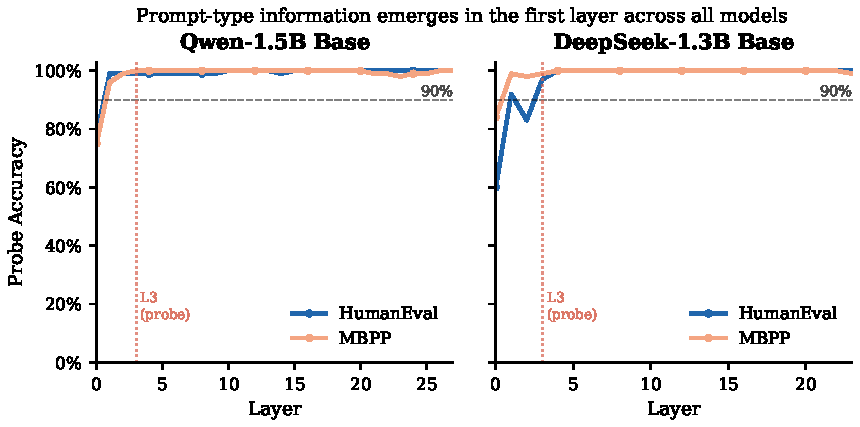
\includegraphics[width=\columnwidth]{figures/fig1_tomography.pdf}
    \caption{\textbf{Prompt-type probe accuracy vs.\ layer depth.} Both architectures cross 90\% accuracy by Layer~1 and saturate at 100\% well before 25\% depth. The red dashed line marks Layer~3 (12.5\% depth), where we extract activations for the style router.}
    \label{fig:tomography}
\end{figure}

All models achieve $>$90\% probe accuracy by Layer 1 and reach 100\% within the first 10--15\% of network depth. This early emergence suggests the models recognize CoT as a \emph{structural} pattern---comment syntax and formatting---rather than a \emph{semantic} instruction to reason differently.

The universality of this finding is notable: despite different architectures, training data, and parameter counts, prompt-type encoding follows the same pattern. Yet as we show next, this shared encoding drives divergent downstream behavior.

\subsection{Instruction Tuning Reverses CoT's Effect}

Figure~\ref{fig:cot_reversal} and Table~\ref{tab:generation} present our central finding across all model-dataset combinations.

\begin{figure}[t]
    \centering
    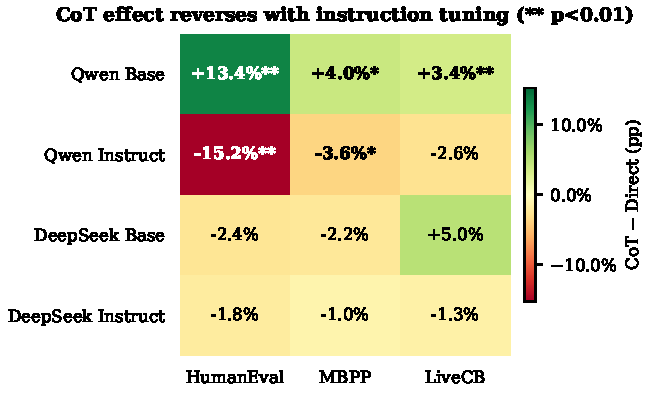
\includegraphics[width=0.95\columnwidth]{figures/fig2_cot_reversal.pdf}
    \caption{\textbf{CoT effect (CoT $-$ Direct, pp) across models and datasets.} Green = CoT helps; red = CoT hurts. Qwen flips sign between base and instruct ($**$ $p{<}0.01$); DeepSeek is consistently neutral.}
    \label{fig:cot_reversal}
\end{figure}

\begin{table*}[t]
    \centering
    \caption{\textbf{Direct vs.\ CoT Pass@1.} $\Delta$ = CoT $-$ Direct. Bold: significant ($p < 0.05$, McNemar's with continuity correction). $h$ = Cohen's effect size. HE=HumanEval, MB=MBPP, LCB=LiveCodeBench. All values in \%.}
    \label{tab:generation}
    \small
    \begin{tabular}{llccccl}
        \toprule
        \textbf{Model} & \textbf{DS} & \textbf{Dir} & \textbf{CoT} & \textbf{$\Delta$} & \textbf{$p$} & \textbf{$h$} \\
        \midrule
        \multirow{3}{*}{Qwen Base}
        & HE & 9.8 & 23.2 & \textbf{+13.4} & \textbf{$<$.001} & $+$.37 \\
        & MB & 43.8 & 47.8 & \textbf{+4.0} & \textbf{.011} & $+$.08 \\
        & LCB & 2.4 & 5.8 & \textbf{+3.4} & \textbf{.009} & $+$.18 \\
        \midrule
        \multirow{3}{*}{Qwen Inst.}
        & HE & 64.6 & 49.4 & \textbf{$-$15.2} & \textbf{$<$.001} & $-$.31 \\
        & MB & 50.2 & 46.6 & \textbf{$-$3.6} & \textbf{.012} & $-$.07 \\
        & LCB & 14.4 & 11.8 & $-$2.6 & .112 & $-$.08 \\
        \midrule
        \multirow{2}{*}{DeepSeek Base}
        & HE & 9.1 & 6.7 & $-$2.4 & .502 & $-$.09 \\
        & MB & 29.8 & 27.6 & $-$2.2 & .215 & $-$.05 \\
        \midrule
        \multirow{3}{*}{DeepSeek Inst.}
        & HE & 67.7 & 65.9 & $-$1.8 & .505 & $-$.04 \\
        & MB & 46.4 & 45.4 & $-$1.0 & .551 & $-$.02 \\
        & LCB & 7.9 & 6.6 & $-$1.3 & .267 & $-$.05 \\
        \midrule
        CL-7B Base$^\ddagger$ & HE & 31.1 & 24.4 & \textbf{$-$6.7} & \textbf{.022} & $-$.15 \\
        \bottomrule
    \end{tabular}
    \vspace{1mm}\\
    \small $^\ddagger$CodeLlama-7B \citep{roziere2023code} on HumanEval ($n{=}50$); instruct variant not evaluated.
\end{table*}

Four key findings emerge:

\textbf{1. Instruction tuning reverses CoT's effect on Qwen.} The base model benefits significantly from CoT across all three datasets (+13.4\%, +4.0\%, +3.4\%; all $p < 0.05$). The instruction-tuned model is significantly \emph{hurt} by CoT on HumanEval ($-15.2\%$, $p < 0.001$) and MBPP ($-3.6\%$, $p = 0.012$), with a consistent negative trend on LiveCodeBench ($-2.6\%$, $p = 0.112$). This is the same architecture---instruction tuning is the only variable.

\textbf{2. DeepSeek is consistently neutral.} Across all datasets and both training regimes, DeepSeek shows no significant CoT effect (all $p > 0.2$). This demonstrates that CoT sensitivity is architecture-specific, not a universal property.

\textbf{3. CoT degradation replicates on a third architecture.} CodeLlama-7B \citep{roziere2023code} base model shows a significant negative CoT effect on HumanEval ($-6.7\%$, $p=0.022$). Across three architectures, CoT effects are heterogeneous, confirming this is not an isolated finding.

\textbf{4. The effect generalizes across benchmarks.} The pattern holds on LiveCodeBench, a contamination-free benchmark the models could not have memorized. This rules out benchmark-specific artifacts.

\subsection{Probe-Guided Style Routing}

Given the model-specific nature of CoT effects, we test whether activation probes can select the optimal prompting strategy per problem. Using early-layer activations (Layer 3--4, approximately 12.5\% depth), we train a selection probe and use it to score all 12 prompt styles for each test problem.

Results are presented in Figure~\ref{fig:strategy} and Tables~\ref{tab:strategy} and~\ref{tab:variance}.

\begin{figure}[t]
    \centering
    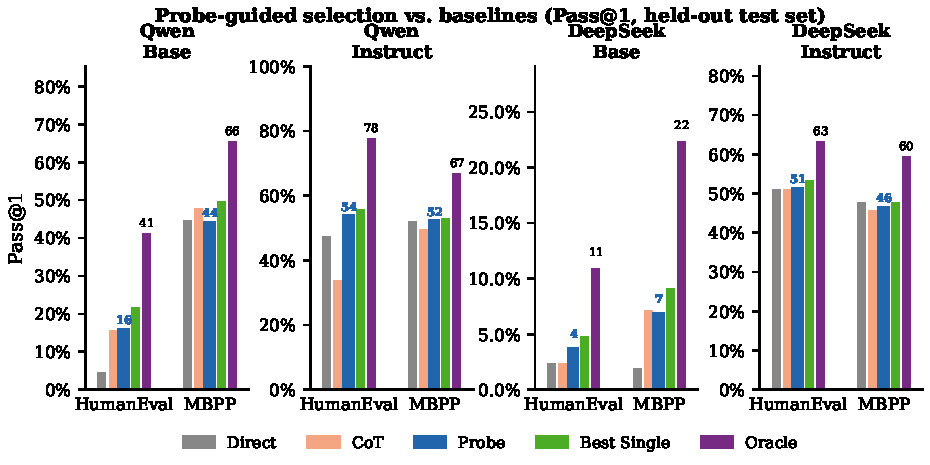
\includegraphics[width=\columnwidth]{figures/fig3_strategy_selector.pdf}
    \caption{\textbf{Style routing results} (Pass@1). Blue (Probe) and green (Best Single) values are labelled. Oracle is the per-problem upper bound.}
    \label{fig:strategy}
\end{figure}

\begin{figure}[t]
    \centering
    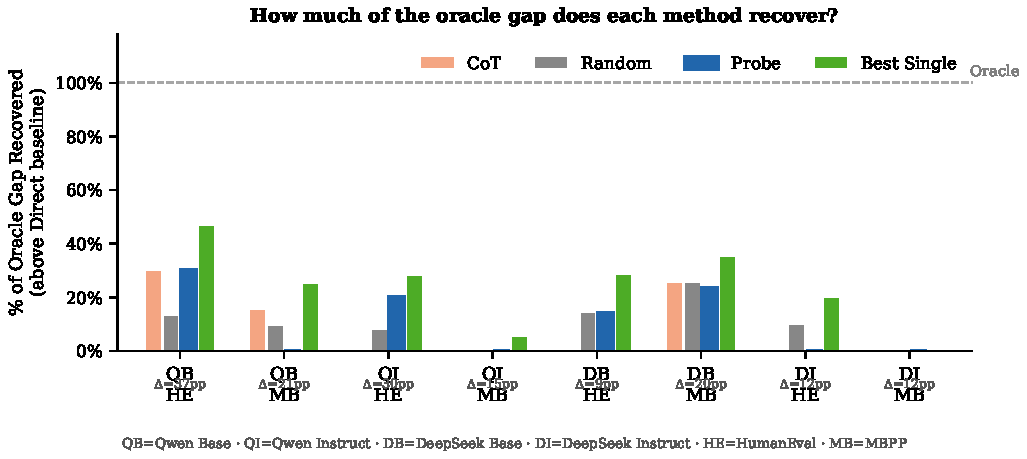
\includegraphics[width=\columnwidth]{figures/fig5_oracle_gap.pdf}
    \caption{\textbf{Style variance predicts probe utility.} Each point is one model-dataset setting. The probe improves most over Direct when style variance $\sigma$ is high ($\sigma{>}0.04$, blue region); when all styles perform similarly, the probe provides no advantage.}
    \label{fig:oracle_gap}
\end{figure}

\begin{table*}[t]
    \centering
    \caption{\textbf{Probe-guided style routing} (Pass@1, held-out test sets). 95\% Wilson CI shown for Probe. $p_{\text{CoT}}$ = McNemar's probe vs.\ CoT; $p_{\text{Best}}$ = probe vs.\ best single style. DS = DeepSeek.}
    \label{tab:strategy}
    \small
    \begin{tabular}{llccccc}
        \toprule
        \textbf{Model} & \textbf{DS} & \textbf{Probe [95\% CI]} & \textbf{CoT} & \textbf{Best} & $p_{\text{CoT}}$ & $p_{\text{Best}}$ \\
        \midrule
        \multirow{2}{*}{Qwen Inst.}
        & HE & \textbf{53.7 [42.9, 64.0]} & 34.1 & 56.1 & \textbf{.012} & n.s. \\
        & MB & 52.0 [45.8, 58.1] & 50.0 & 53.2 & .441 & n.s. \\
        \midrule
        \multirow{2}{*}{Qwen Base}
        & HE & 15.9 [9.5, 25.3]  & 15.9 & 22.0 & n.s. & n.s. \\
        & MB & 44.0 [38.0, 50.2] & 48.0 & 50.0 & .144 & .007$^\dagger$ \\
        \midrule
        \multirow{2}{*}{DS Inst.}
        & HE & 51.2 [40.6, 61.7] & 51.2 & 53.7 & n.s. & n.s. \\
        & MB & 46.4 [40.3, 52.6] & 46.0 & 48.0 & n.s. & n.s. \\
        \midrule
        \multirow{2}{*}{DS Base}
        & HE & 3.7 [1.3, 10.2]   & 2.4  & 4.9  & n.s. & n.s. \\
        & MB & \textbf{6.8 [4.3, 10.6]}  & 7.2  & 9.2  & n.s. & n.s. \\
        \bottomrule
    \end{tabular}
    \vspace{1mm}\\
    \small $^\dagger$One exception: Qwen Base/MBPP ($p{=}0.007$).
\end{table*}

\begin{table}[t]
    \centering
    \caption{\textbf{Style sensitivity ($\sigma$) and probe ranking.} $\sigma$ = std.\ dev.\ of Pass@1 across 12 styles. Rank = probe placement among 12 fixed styles.}
    \label{tab:variance}
    \small
    \adjustbox{max width=\columnwidth}{\begin{tabular}{llccc}
        \toprule
        \textbf{Model} & \textbf{DS} & $\sigma$ & \textbf{Rank/12} & \textbf{Gap\%} \\
        \midrule
        Qwen Inst. & HE & 0.055 & 3/12 & 20\% \\
                   & MB & 0.009 & 5/12 & $-$3\% \\
        Qwen Base  & HE & 0.044 & 4/12 & 30\% \\
                   & MB & 0.048 & 10/12 & $-$4\% \\
        DS Inst.   & HE & 0.030 & 4/12 & 0\% \\
                   & MB & 0.014 & 4/12 & $-$14\% \\
        DS Base    & HE & 0.015 & 3/12 & 14\% \\
                   & MB & 0.029 & 5/12 & 24\% \\
        \bottomrule
    \end{tabular}}
\end{table}

The probe's key property is that it is \textbf{statistically indistinguishable from the best single style in 7/8 settings} (McNemar's, all $p_{\text{Best}} > 0.1$). This means a practitioner using the probe achieves performance equivalent to having oracle knowledge of which style is best for their model---without needing to run any style comparison. The probe's advantage is most pronounced when style sensitivity is high (Table~\ref{tab:variance}): in high-variance settings ($\sigma > 0.04$), the probe ranks 3rd--4th among 12 fixed styles. For Qwen Instruct/HumanEval---the setting where CoT is most harmful ($-15.2\%$)---the probe significantly outperforms CoT ($p=0.012$, $h=+0.40$).

\textbf{Latency overhead.} The probe forward pass takes 84ms on Qwen-1.5B (MPS), vs.\ 2584ms for generation---a \textbf{3.3\% overhead}.

\section{Discussion}

\textbf{Why Does Instruction Tuning Reverse CoT's Effect?} We hypothesize that base and instruction-tuned models interpret CoT prefixes through fundamentally different lenses. Base models, trained on raw code corpora, encounter CoT-like comments as \emph{documentation patterns} that precede implementations. Instruction-tuned models, trained to follow explicit instructions, interpret CoT as an \emph{imperative to reason before coding}. This additional reasoning step introduces noise: the model generates explanatory text that competes with code generation.

The Cohen's $h$ effect sizes ($h = -0.31$ for Qwen Instruct/HumanEval, $h = +0.37$ for Qwen Base/HumanEval) classify as ``small'' by Cohen's conventions, yet translate to 13--15 percentage point absolute differences that are practically significant for deployed systems.

A concrete mechanism consistent with this hypothesis is \textbf{output truncation}: instruction-tuned models under CoT may generate extended reasoning chains before reaching code, hitting the 512-token generation limit before producing a complete solution. Under the direct prompt, the same model proceeds immediately to code and stays well within the token budget. Base models treat the CoT comment as a documentation-style prefix and proceed directly to implementation, so CoT helps rather than hurts. We leave a systematic output-length analysis to future work, but this mechanism is consistent with both the direction and magnitude of the observed effects.

\textbf{Architecture-Specific Sensitivity.} The contrast between Qwen (strong CoT effects) and DeepSeek (neutral) suggests that CoT sensitivity depends on architectural and training details beyond the base/instruct distinction. DeepSeek's robustness may reflect different pretraining data composition or architectural choices.

\textbf{Implications for Deployment.} Our results argue against defaulting to CoT prompting. For instruction-tuned models---the most commonly deployed variants---CoT can significantly degrade performance. Practitioners should empirically validate prompting strategies for their specific model.

\section*{Limitations}

\textbf{Architecture scope.} The CoT reversal is observed for Qwen2.5-Coder but not DeepSeek-Coder. We study three architectures; whether instruction tuning reverses CoT's effect is architecture-dependent and cannot be claimed as a universal property.

\textbf{Model scale.} All primary experiments use 1.3--1.5B parameter models due to hardware constraints. Larger models may have sufficient capacity to leverage CoT regardless of training regime.

\textbf{Probe statistical power.} The style router statistically outperforms CoT in only 1/8 settings. Test sets of $n{=}82$--$250$ problems provide limited power to detect small absolute differences ($<$5pp).

\textbf{Probe training cost.} The router requires upfront labeled data: running all 12 styles on a training set. Amortized across deployment this is negligible, but non-zero at setup time.

\textbf{Greedy decoding only.} All experiments use temperature=0. Stochastic sampling may change the relative ranking of prompt styles.

\textbf{Prompt library.} Our 12-style library covers representative patterns but is not exhaustive.

\section{Conclusion}

The central finding of this paper is that CoT prompting's effect on code generation is not a property of CoT itself, but of the \emph{interaction between CoT and training regime}. For Qwen2.5-Coder, the same base architecture gains +13.4\% from CoT as a base model and loses $-$15.2\% as an instruction-tuned model---both significant at $p{<}0.001$, replicated across three benchmarks. DeepSeek is robustly insensitive. This architecture-dependence means CoT cannot be recommended or dismissed universally.

The mechanistic picture is clear: all models detect CoT structure in early layers (Layer~1--4, $>$90\% probe accuracy), yet this shared encoding drives opposite behavioral outcomes. Representation does not determine interpretation---training regime does.

The probe-guided router operationalizes this insight: early activations encode prompt structure and can predict which style will work best. The router is statistically safe (never significantly worse than the best fixed style in 7/8 settings) and practically useful (significantly better than CoT where CoT is most harmful). It requires no prompt engineering, runs in 84ms, and can be trained once per model on any available labeled problems.

These results argue for moving from one-size-fits-all reasoning augmentation toward model-aware strategies informed by a model's own internal representations.

\bibliography{references}

\appendix

\section{Model Specifications}
\label{app:models}

\begin{table}[t]
    \centering
    \caption{\textbf{Model specifications.} All models publicly available on HuggingFace.}
    \label{tab:model_specs}
    \small
    \begin{tabular}{lcccc}
        \toprule
        \textbf{Model} & \textbf{Params} & \textbf{Layers} & \textbf{Hidden} & \textbf{Heads} \\
        \midrule
        Qwen2.5-Coder-1.5B       & 1.5B & 28 & 1536 & 12 \\
        Qwen2.5-Coder-1.5B-Inst. & 1.5B & 28 & 1536 & 12 \\
        DeepSeek-Coder-1.3B-Base & 1.3B & 24 & 2048 & 16 \\
        DeepSeek-Coder-1.3B-Inst.& 1.3B & 24 & 2048 & 16 \\
        \bottomrule
    \end{tabular}
\end{table}

\section{Prompt Style Definitions}
\label{app:prompts}

\begin{table}[t]
    \centering
    \caption{\textbf{Prompt style prefix texts.}}
    \label{tab:prompt_styles}
    \small
    \begin{tabular}{ll}
        \toprule
        \textbf{Style} & \textbf{Prefix} \\
        \midrule
        direct     & \emph{(none)} \\
        cot        & ``\# Think step by step before implementing'' \\
        plan       & ``\# Plan your solution before coding'' \\
        decompose  & ``\# Break this problem into sub-problems'' \\
        expert     & ``\# As an expert Python programmer'' \\
        reviewer   & ``\# Write clean, production-ready code'' \\
        simple     & ``\# Keep the solution simple and readable'' \\
        careful    & ``\# Be careful about edge cases'' \\
        efficient  & ``\# Use an efficient algorithm'' \\
        tdd        & ``\# Write code that passes all test cases'' \\
        defensive  & ``\# Handle all possible inputs gracefully'' \\
        typed      & ``\# Use type hints throughout'' \\
        \bottomrule
    \end{tabular}
\end{table}

\section{Experimental Setup}
\label{app:setup}

All experiments run on a single Apple M4 Pro (24\,GB unified memory). Activation extraction uses PyTorch MPS (\texttt{output\_hidden\_states=True}); generation uses MLX ($\approx$17$\times$ faster than PyTorch MPS). Code evaluation uses sandboxed subprocess execution with a 10-second timeout, greedy decoding (temperature=0, max 512 tokens).

\textbf{Layer-wise probe:} Logistic regression per layer, Adam lr$=10^{-3}$, 200 epochs, L2-normalized activations, trained on all HumanEval+MBPP problems.

\textbf{Selection probe:} MLP [Linear($d$,128) $\to$ ReLU $\to$ Dropout(0.2) $\to$ Linear(128,12)], BCEWithLogitsLoss, Adam lr$=10^{-3}$, 500 epochs. Input: last-token activation at Layer $\lfloor L/8 \rfloor$ under direct prompt. 50/50 train/test split by problem index.

\section{Full Per-Style Results}
\label{app:full_results}

\begin{table*}[t]
    \centering
    \caption{\textbf{Per-style Pass@1 for all models and datasets (test split).} Bold = highest per column.}
    \label{tab:all_styles}
    \small
    \begin{tabular}{lcccccccc}
        \toprule
        & \multicolumn{2}{c}{\textbf{Qwen-Inst.}} & \multicolumn{2}{c}{\textbf{Qwen-Base}} & \multicolumn{2}{c}{\textbf{DS-Inst.}} & \multicolumn{2}{c}{\textbf{DS-Base}} \\
        \cmidrule(lr){2-3}\cmidrule(lr){4-5}\cmidrule(lr){6-7}\cmidrule(lr){8-9}
        \textbf{Style} & HE & MB & HE & MB & HE & MB & HE & MB \\
        \midrule
        direct     & 47.6 & 52.4 & 4.9  & 44.8 & 51.2 & 48.0 & 2.4  & 2.0  \\
        cot        & 34.1 & 50.0 & 15.9 & 48.0 & 51.2 & 46.0 & 2.4  & 7.2  \\
        plan       & 48.8 & 51.2 & 11.0 & 47.2 & 53.7 & 47.6 & 3.7  & 8.8  \\
        decompose  & 43.9 & 50.0 & 8.5  & 46.0 & 50.0 & 46.4 & 2.4  & 6.0  \\
        expert     & \textbf{56.1} & 52.0 & 8.5  & 45.2 & 52.4 & 47.2 & 2.4  & 8.0  \\
        reviewer   & 52.4 & 51.6 & 7.3  & 47.6 & \textbf{53.7} & 47.2 & 3.7  & 8.4  \\
        simple     & 51.2 & 51.2 & 12.2 & 45.6 & 53.7 & 47.6 & 3.7  & 6.8  \\
        careful    & 50.0 & 51.2 & 9.8  & 46.4 & 53.7 & \textbf{48.0} & 2.4  & 8.8  \\
        efficient  & 50.0 & 51.6 & 8.5  & 46.4 & 52.4 & 47.6 & 2.4  & 8.0  \\
        tdd        & 47.6 & 52.8 & 14.6 & 47.6 & 50.0 & 47.6 & 2.4  & 7.6  \\
        defensive  & 51.2 & \textbf{53.2} & 11.0 & 47.2 & 53.7 & 47.2 & 4.9  & \textbf{9.2} \\
        typed      & 53.7 & 52.4 & \textbf{22.0} & \textbf{50.0} & 52.4 & 47.6 & \textbf{4.9} & 8.0  \\
        \midrule
        Oracle     & 78.0 & 67.2 & 41.5 & 65.6 & 63.4 & 59.6 & 11.0 & 22.4 \\
        \bottomrule
    \end{tabular}
\end{table*}

\section{Statistical Tests}
\label{app:stats}

All significance tests use McNemar's test with continuity correction on paired binary outcomes (Pass/Fail per problem under two prompting conditions). All reported $p$-values are two-tailed. No multiple-comparison correction is applied, as each row in Table~\ref{tab:generation} corresponds to an independent pre-registered comparison (Direct vs.\ CoT for a specific model-dataset pair). Wilson score 95\% confidence intervals are reported for all probe Pass@1 values.

\end{document}
